\documentclass{article}
\usepackage[utf8]{inputenc}

\usepackage{amsthm}
\usepackage{amsmath}
\newtheoremstyle{mystyle}% name
  {\topsep}% Space above
  {\topsep}% Space below
  {\normalfont}% Body font
  {}% Indent amount
  {\bfseries}% Theorem head font
  {}%Punctuation after theorem head
  {.5em}%Space after theorem head
  {}% theorem head spec
\theoremstyle{mystyle}
\newtheorem{prob}{Problem}
\usepackage{graphicx}
\usepackage{wrapfig}


\title{EN.520.216 Homework 2}
\author{LJ Gonzales}
\date{February 2023}

\begin{document}
\maketitle

\begin{prob}
	\begin{enumerate}
		\item First notice that the voltage at the anode of D4 is 0.6V (0V ground+dropoff voltage), and likewise the voltages at the anodes of D1, D2, and D3 are 1.2V, 0.9V, and 0.9V respectively. This is when we use the first-order model where a diode is considered to be a source with the positive terminal on the side opposing current flow.
		Because the supply voltage is maintained at 18V, it follows that the respective currents are $I_1=\frac{18-1.2}{2200}= 7.63mA$, $I_2=\frac{18-0.9}{2700}= 6.33mA$, and $I_3=\frac{18-0.9}{1000}= 17.1mA$.
		By Kirchoff's law the current through the source is then 31.06mA.
	
	\item All of the diodes are forward-biased, since the voltage at the anode is lower than the voltage at the cathode.

	\item The power absorbed by D4 can be computed from $P=IV$ where I and V are the current and voltage through the component. Using $I_d$ and 0.6V we get $P= 18.636mW$.
	\end{enumerate}
\end{prob}

\begin{prob}
	\begin{enumerate}
	\item
		\begin{tikzpicture}
\draw[gray] plot [smooth] coordinates {(0,1) (2,1) (3,0) (6,0)};
\draw[gray] plot [smooth] coordinates {(0,3) (2, 3) (3,2) (6,2)};
\draw[gray, dashed]	(0,1.5) -- (6,1.5);
\node[right] at (6,2) {$E_{c,n}$};
\node[right] at (6,1.5) {$E_{f}$};
\node[right] at (6,0) {$E_{v,n}$};
\node[left] at (0,3) {$E_{c,n}$};
\node[left] at (0,1) {$E_{v,p}$};
\node[right] at (0,-1) {P region};
\node[left] at (6,-1) {N region};
	\end{tikzpicture}
\item We consider that the valence level in the n-type region opposing the junction has 0 energy relative to the rest of the system, and thus an intrinsic fermi level of $\frac{1}{2}(1.1)= 0.55$ eV.
	We can then use a straight application of the formula $\ln(\frac{n_i}{n_d})=\frac{-\Delta E}{kT}$ with $n\approx N_D=8\times10^{16}$ to find the shift of the fermi energy relative to that intrinsic fermi level. We find this to be 0.38eV.
	The fermi level is then at 0.93eV. 

\item The contact potential is given by $\Phi \ln{\frac{N_AN_D}{n_i^2}}$ where $\Phi =\frac{kT}{q} \approx 26mV$ at 300K. This means that $V_o$ for this particular junction is about 0.837V.
	
\end{enumerate}
\end{prob}
\begin{figure}[h]
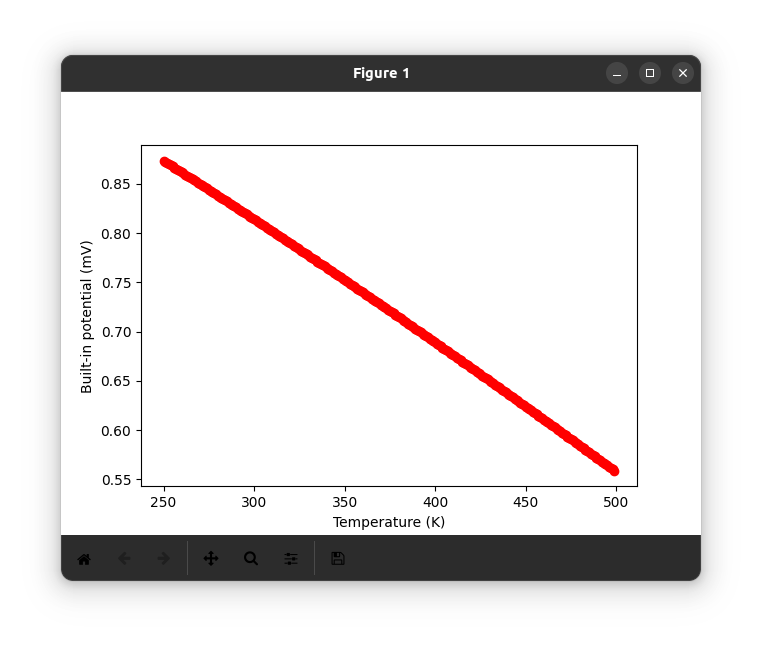
\includegraphics[width =0.7\textwidth]{Screenshot from 2023-02-21 12-47-15.png}
	\label{grappph}
	\caption{Temperature vs. built-in voltage}
\end{figure}

\begin{prob}
	\begin{enumerate}
		\item No, the diode is not always forward biased. For example, when the sinusoid goes negative, the diode is always going to be reversed biased.

		\item The diode makes sure that only current in the positive direction goes through the load.
			The capacitor makes sure that a positive voltage is at least partially maintained through the load even when the source tries to pull current the other way (where usually there would be no current through the resistor thanks to the diode).

	\item We first note that the saturation current of this diode vastly diverges from the one we would expect from a silicon diode so we can't make a direct assumption about its voltage drop (e.g 0.7V). \\
		Instead we find the value of R in terms of $V_{DOn}$ and subsequently estimate its value.
		The circuit can be partitioned in two periods of operation: a) while the diode is in forward conduction (mostly on the rising of the voltage source) and b) when the diode is reversed biased, and the load just sees a capacitor discharging through it. \\
	We can make the assumption that the diode enters reverse bias as soon as the voltage source reaches its peak (if the capacitor-resistor system discharges faster than the source goes down, we wouldn't see any ripple at all, just a half-rectified wave).
		Hence, the time period that the capacitor discharges through the load resistor (with no help from the voltage source) is [$\frac{1}{4}T, t_1]$, where T is the period of the sinusoid and $t_1$ is the timestamp at which the diode is back in forward conduction. \\
		We know $t_1$ to satisfy  $\sin{20\pi t_1}=V_{DOn}$, and the first time that the diode comes back up is given by  $t_1=\frac{1}{20\pi}\sin ^{-1}(V_{DOn})+\frac{1}{10}$. (adding the length of one period).
		Further, we want to make sure that during that period, the voltage across the load does not decrease more than $1-V_{DOn}-0.5$, from its original value of $1-V_{DOn}$.
		We know the differential equation of an RC circuit:
		\begin{align*}
			\int _{t=\frac{1}{4}T}^{\frac{1}{20\pi}\sin ^{-1}(V_{DOn})+\frac{1}{10}}\frac{1}{RC}dt = \int _{1-V_{DOn}-0.5}^{1-V_{DOn}}\frac{1}{V_c(t)}dV_c(t) \\
			\therefore R= \frac{\frac{1}{20\pi}\sin ^{-1}(V_{DOn})+ \frac{3}{40}}{10\times10^{-6}\ln \big(\frac{1-V_{DOn}}{1-V_{DOn}-0.5}\big)}
		\end{align*}
		\begin{wrapfigure}{L}{0.4\textwidth}
			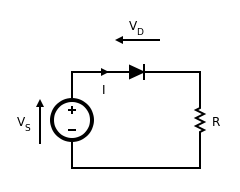
\includegraphics[width = 0.4\textwidth]{diodemodelling.png}
		\end{wrapfigure}

		Just as we did to obtain the 0.7V estimation of the silicon diode, we can set up a voltage source, diode, and resistor in series and solve under the exponential model to get $V_{DOn}$ (see figure below). With a 1V source and 10k$\Omega$ resistor, we have
		$1-V_{DOn}-1.8\times10^{-2}(e^{V_{DOn}/\Phi_T}-1)=0$, which gives a $V_{DOn}$ value of 0.103V. In fact, choosing other values of V and R changes the result very little. 
				
		Putting this back in the equation, we get $R\approx9402\Omega$, our final answer. \\
	\item The maximum output voltage under the constant drop model is given by the max source voltage minus one voltage drop, or about 0.897V
	
	\item \begin{figure}[h]
		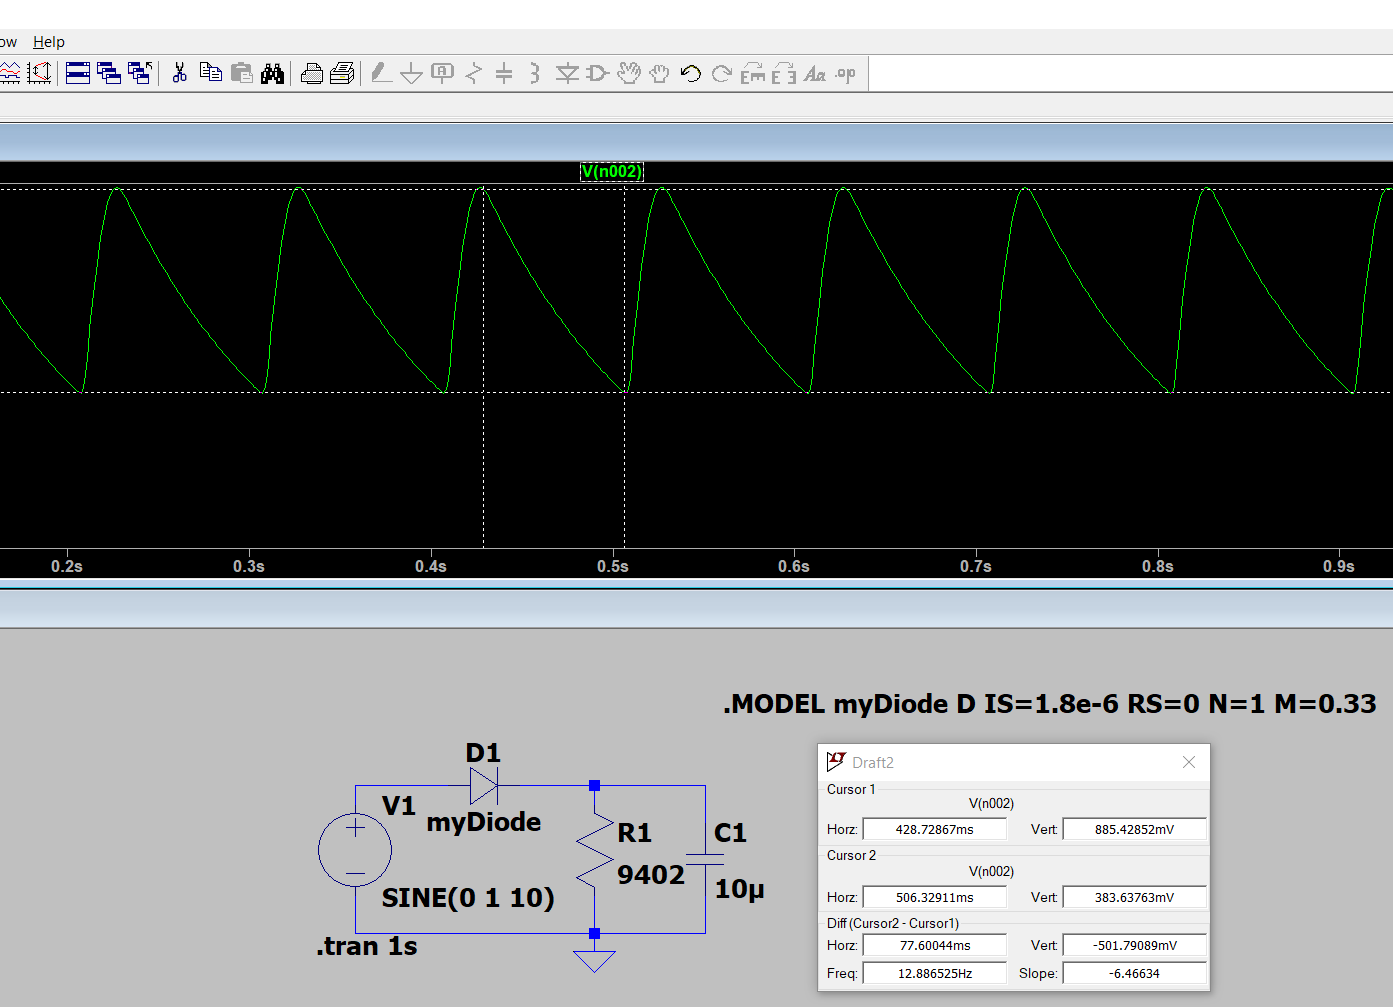
\includegraphics[width =\textwidth]{Capture.png}
		\label{ltspice}
		\caption{LTSpice Simulation}
	\end{figure}
	
	\end{enumerate}
\end{prob}
\end{document}
